\section{User Centered Studies} \label{sec:userstudies}

Firstly, developing this kind of technology, such as a robot for aged people, brings some delicate questions.
The potential users sometimes have few or nonexistent experience with technology.
Regarding this evidence, it is difficult for them to understand how robots work and what can they actually do.

Considering the goals of this project, it will require user studies, similarly to what Pereira et al. have done with the Risk player.
These user studies aim to collect specific behaviours and verbal interactions in the domain of \emph{Sueca}.
However, understanding their needs, expectations and fears is a priority. As a result, it was developed a pilot study in a care home in order to answer all these questions.

The pilot study involved two different
activities, a focus group and a card game.
This branching was a result of two distinct motivations, understanding the elderly' concerns about robots and collecting information in the game domain.





\subsection{Focus Group}
The focus group firstly aims to introduce the team.
It is important to establish a connection with this care home for further studies.
This kind of user study also seems to be a good approach for a first meeting due to the informal and conversational way of interacting with them.
Usually, people tend to feel comfortable and easily share their opinions about the topic being discussed.

\subsubsection{Methodology}
The elderly participants were divided into groups of 5 people.
There were 2 researchers per group commanding and guiding all the process.
The list of used materials is:

\begin{itemize}
\item A video to illustrate what is a robot;
\item Photographies of different robots (including the service and companion types);
\item Two white boards and three pens (black, red and green);
\item Three hypothetical stories of robots;
\item An audio recorder;
\item A video camera.
\end{itemize}

The two last items were only used for a further analyses of this focus group.
The mentioned video tries to answer the questions: what is a robot, what can robots do, how do they work, do they fail and how do science fiction movies present robots to us.
In order not to bias their thoughts, we tried to gather positive and negative aspects of existing robots.
The three hypothetical stories aim to bring ethical discussions to the focus group.
For instance, an elderly that owns a robot in his home tells him a secret.
If that robot is questioned about the secret, it should or should not tell other people the truth?

\subsubsection{Procedures}
All the material enumerated in the previous list were arranged as in the Figure~\ref{fig:focus-group}.
Firstly, each one in the room briefly introduces himself in order to make everyone feeling more comfortable.
Secondly, the video is shown.
Then, everyone starts discussing about robots' purposes and they are registered in one of the white boards with the black coloured pen.
People also express a positive or negative impression of each robot's purpose and it decides the colour of the surrounding line around the idea.
For instance, the sentence ``Call an ambulance'' wrote on the board is surrounded by a green line if they think it is a good purpose for a robot.
After finishing this task, one of the group leaders writes all the sentences previously collected in the second board but without the surrounding green or red lines.
The other group leader starts reading the hypothetical stories and opens a new discussion about what should the robots of each story do.
He also presents the photographies and try to understand which robot is more suitable for each purpose in their opinion.
When bringing the new board to the room, the idea is to understand if their positive and negative opinions about each purpose have changed.

\begin{figure}
        \centering
        \begin{subfigure}[h]{0.49\textwidth}
                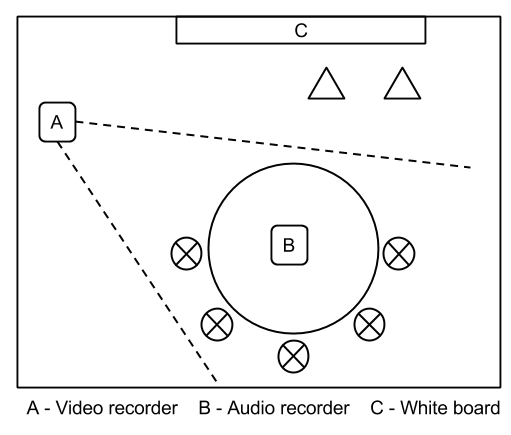
\includegraphics[width=\textwidth]{./img/focusGroup}
                \caption{Focus Group}
                \label{fig:focus-group}
        \end{subfigure}
        \begin{subfigure}[h]{0.49\textwidth}
                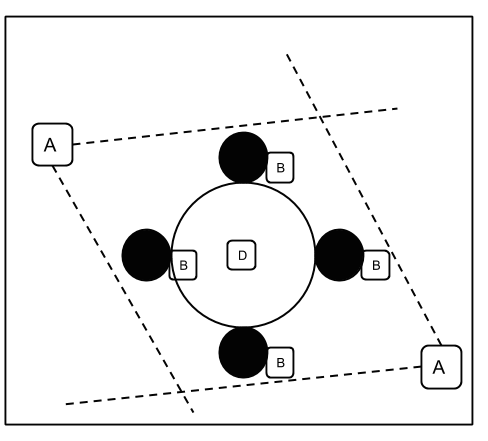
\includegraphics[width=\textwidth]{./img/cardGame}
                \caption{Card game}
                \label{fig:card-game}
        \end{subfigure}
        \caption{Setting of the user study activities}\label{fig:user-studies}
\end{figure}


\subsubsection{Preliminary Results}

This focus group is an on going activity that has not been fully analysed.
It has already been collected information from 3 different focus groups with a sum of 15 participants.
For instance, contrasting with what was expected, the elderly do not feel uncomfortable and disrespected with a robot calling the doctor and revealing improper behaviours from its owner.
Instead, they think it is a valuable aid in their lives and might save them while disrespecting strict instructions.
In addition, their safety is their prior worry.
When walking through the house and sometimes due to physical disabilities, they fear about falling and not being noticed.







\subsection{Card Game}
This pilot activity with a card game aims to understand difficulties for further studies.
For instance, lightning conditions might affect video recording or the room acoustic and noise might affect audio recording.
Testing this conditions is essential to guarantee the analyses of further studies.
It also aims to start collecting information from the \emph{Sueca} domain.
This means perceiving how they play, what do players say and how they behave in certain game states.

\subsubsection{Methodology}
Recording each \emph{Sueca} card game requires four players, one card deck, a table and chairs for the four players, two video cameras and an audio recorder with four microphones.

\subsubsection{Procedures}
All the material previously enumerated were arranged as in the Figure~\ref{fig:card-game}.
Each video camera is positioned in a way that can capture the hands of two adjacent players.
Players were recorded during a tournament of several games.
They were told to play as long as they want with a maximum duration of one hour.

\subsubsection{Preliminary Results}
\todo{Watch videos and complete this section}





% necessidade de perceber se sao aceites quer por utilidade quer por companhia e fazer referenca a heerink evers e wielinga


% Kerstin Dautenhahn  et. al. introduced in 2013 the \gls{thri}, that aims to integrate theatre into user studies.
% Since \gls{vhri} does not provide live experiences, this new methodology is considered more immersive.
% Their last \gls{thri} study has been done in an elderly care home and its purpose was analysing both residents and carers' opinions.
% The results and conclusions of the mentioned user study revealed a problem with questionnaires.
% Due to the ageing-associated disorders, such as poor eyesight or arthritis in hands, part of the users could not answered the questionnaires.
% However, seniors' opinion about robots have been compared with their previous \gls{thri} with children.
% The younger related to robots as pets or servants.
% On the other hand, elderly related them as companions or friends.
% This evidence might suggest a feeling of loliness and the lack of company.

